\section{Các cú pháp đã hỗ trợ}

Phần này sẽ trình bày một số cú pháp của Rust khác biệt so với ngôn ngữ C/C++ và cách mà công cụ đã hỗ trợ cho các cú pháp này.
Các cú pháp bao gồm: if let, while let, match, lifetime.
Những đoạn mã nguồn và hình ảnh mô tả đồ thị CPG được sử dụng từ giờ đến cuối chương đã được đơn giản hóa để dễ dàng thể hiện và minh họa.
Các cạnh và các nút không phải trọng tâm của đồ thị CPG đã được loại bỏ để tập trung vào các tính năng cần trình bày.

\subsection{Cú pháp if let}
If else là cấu trúc điều khiển có mặt trong tất cả các loại ngôn ngữ phổ biến.
Nó cho phép chúng ta kiểm tra một điều kiện và thực thi một khối mã nếu điều kiện đúng và một khối mã khác nếu điều kiện sai.
Cấu trúc câu lệnh if else sẽ bao gồm một điều kiện và 2 khối mã.
Nếu điều kiện đúng, khối mã trong if sẽ được thực thi, ngược lại khối mã trong else sẽ được thực thi.
Thông thường khối điều kiện sẽ là biểu thức trả về kết quả đúng hoặc sai của biểu thức đó.
Trong ngôn ngữ như C/C++ thì chỉ chấp nhận biểu thức điều kiện, việc sử dụng mệnh đề có dấu hai chấm để kết thúc câu lệnh là không hợp lệ.

Với phương châm \textit{"Expression over statement"} và nhằm mục đích tạo sự ngắn gọn, Rust cho phép thực hiện phép khai báo biến và gán giá trị cho biến trong cùng một câu lệnh bằng điều kiện if let.
Cú pháp của câu lệnh if let như sau:

\begin{minted}[mathescape, breaklines, frame=lines, framesep=2mm, baselinestretch=1.2, fontsize=\footnotesize, linenos]{rust}
if let <pattern> = <expression> {
     <block>
} else {
     <block>
}
\end{minted}

\usemintedstyle{default}

Cú pháp này sẽ thực hiện 2 công việc, kiểm tra xem \texttt{<expression>} có khớp với \texttt{<pattern>} hay không, nếu không khớp thì trả về $false$, nếu có khớp thì tiếp tục thực hiện tạo biến mới dựa theo \texttt{<pattern>} vừa lấy được và trả về $true$.
Các biến được khai báo mới từ \texttt{<pattern>} sẽ có phạm vi tồn tại trong khối lệnh điều kiện thành công.
Do thực hiện 2 công việc trong cùng 1 câu lệnh nên khi quy đổi sang câu lệnh tương tự trong ngôn ngữ như C/C++ sẽ tương đương 2 câu lệnh kiểm tra điều kiện và gán biến.

\begin{listing}[H]
\begin{minted}[mathescape, breaklines, frame=lines, framesep=2mm, baselinestretch=1.2, fontsize=\footnotesize, linenos]{rust}
let number: Option<i32> = None;
let i_like_letters = false;

if let Some(i) = number {
    println!("Matched number {:?}!", i);
} else if i_like_letters {
    // ...
} else {
    // ...
}
\end{minted}
\caption{Ví dụ mã nguồn cho if let}
\label{code:c4_iflet}
\end{listing}

\begin{listing}[H]
\begin{minted}[mathescape, breaklines, frame=lines, framesep=2mm, baselinestretch=1.2, fontsize=\footnotesize, linenos]{cpp}
Object* obj = inputObj();

if (obj != nullptr) { // 1 câu lệnh kiểm tra điều kiện
    int number = *static_cast<int*>(obj); // 1 câu lệnh gán biến
    std::cout << "Matched " << number << "!" << std::endl;
}
\end{minted}
\caption{Ví dụ mã nguồn cho if let tương đương trong C++}
\label{code:c4_iflet_cpp}
\end{listing}

Trong hình \ref{img:c4_cpg_iflet}, cạnh \texttt{CONDITION} của nút \texttt{ExprIf} trỏ tới nút \texttt{Assignment}, đồng thời cũng khai báo biến mới với tên $i$.
Mặc định Joern sẽ không cho phép cạnh \texttt{CONDITION} tới nút \texttt{Assignment} bởi vì trong ngôn ngữ C/C++ không lấy một phép gán làm điều kiện cho câu lệnh if.
Khóa luận đã thực hiện chỉnh sửa đặc tả CPG của Joern để cho phép cạnh \texttt{CONDITION} trỏ tới nút \texttt{Assignment} trong trường hợp này.
Các mệnh đề trong khối được thực thi khi điều kiện đúng nếu có nhắc tới biến $i$ thì sẽ tham chiếu tới biến $i$ vừa được khai báo thông qua cạnh \texttt{REF}.

\begin{figure}[H]
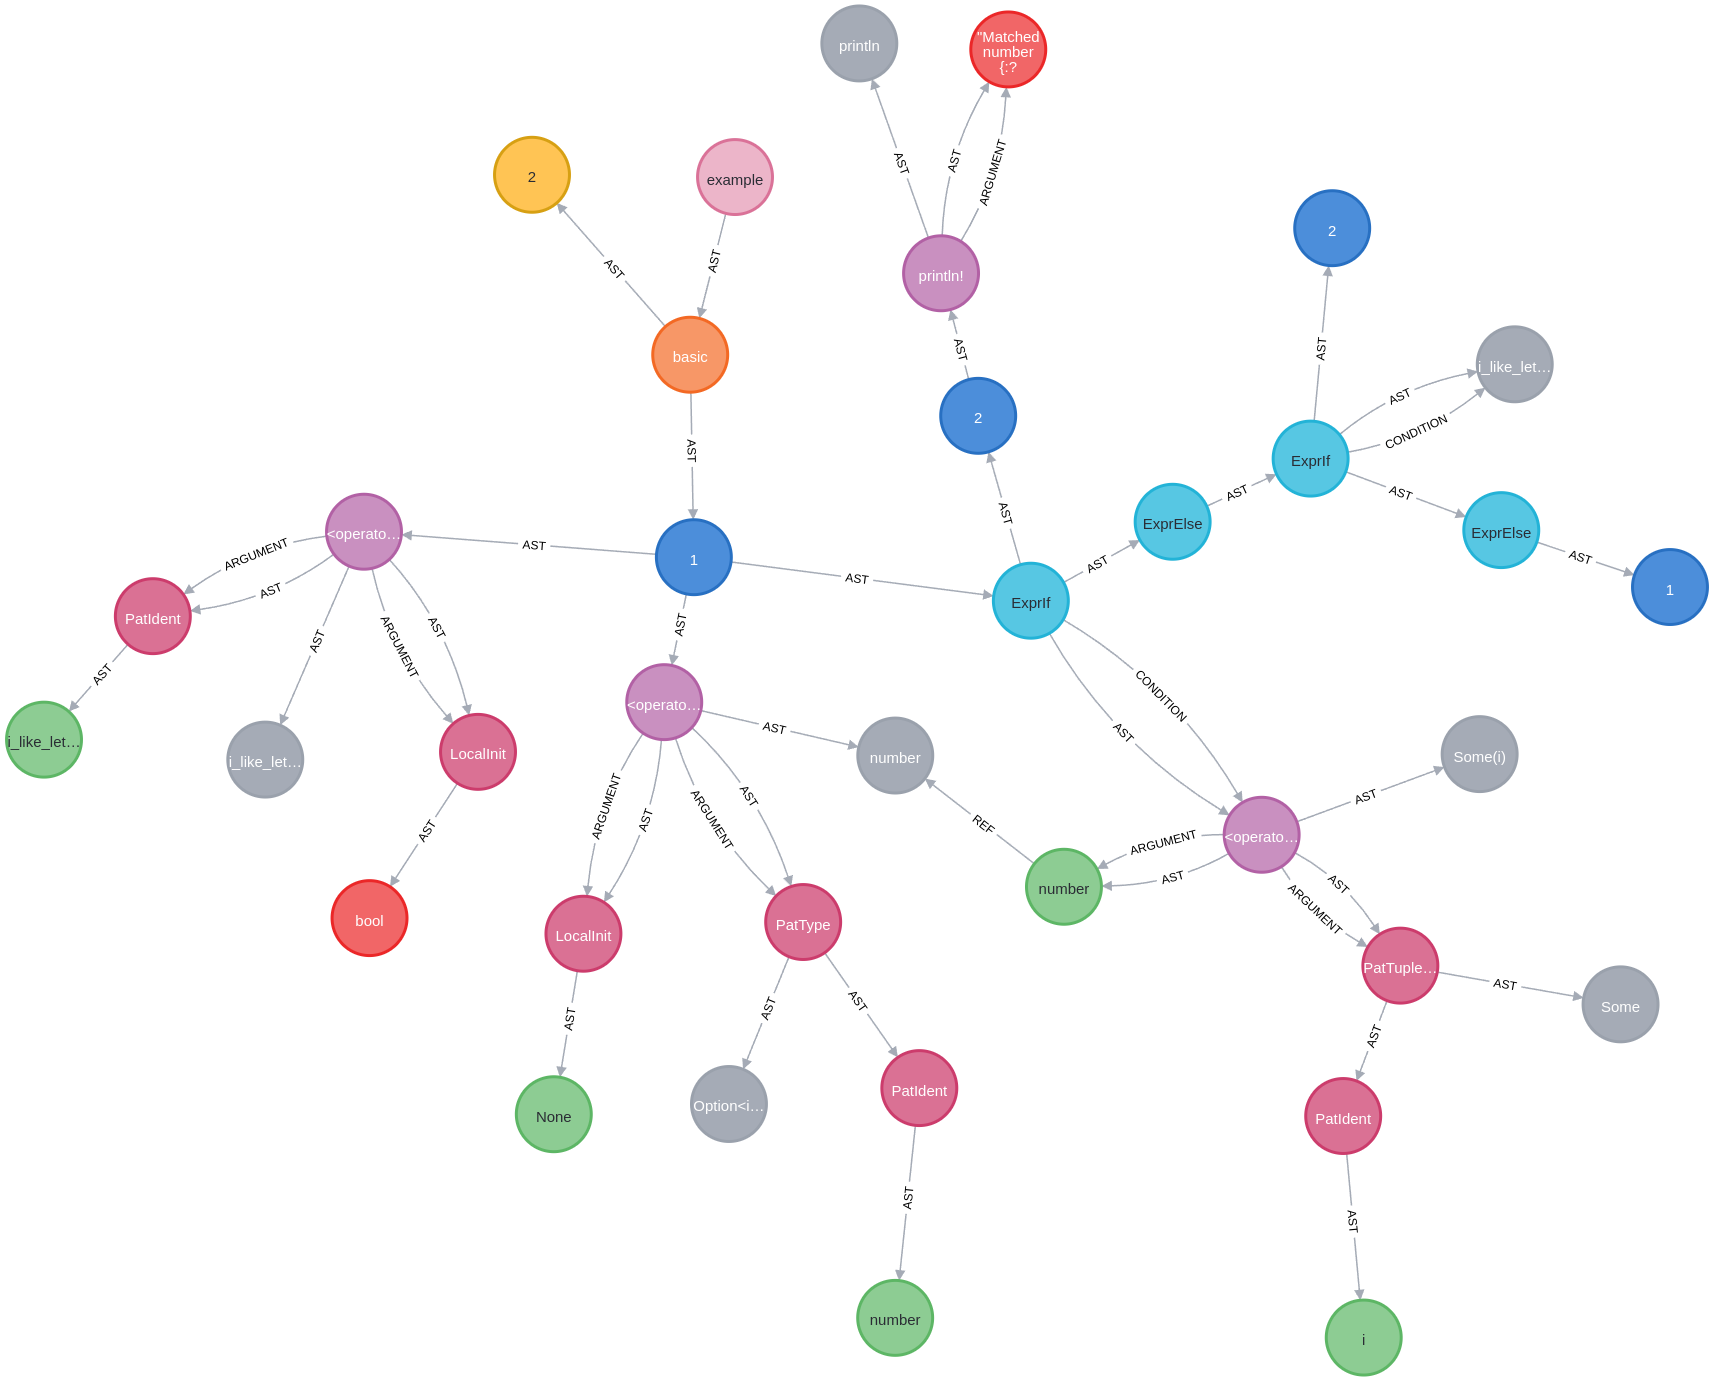
\includegraphics[width=1\columnwidth]{figures/c4/c4_iflet.png}
\centering
\caption{Ví dụ đồ thị CPG cho đoạn mã nguồn if let \ref{code:c4_iflet}}
\label{img:c4_cpg_iflet}
\end{figure}

\subsection{Cú pháp while let}

Tương tự với tính năng if let ở trên, Rust cũng hỗ trợ việc khai báo biến làm điều kiện cho vòng lặp while. Cú pháp của vòng lặp while let như sau:

\begin{minted}[mathescape, breaklines, frame=lines, framesep=2mm, baselinestretch=1.2, fontsize=\footnotesize, linenos]{rust}
while let <pattern> = <expression> {
        <block>
}
\end{minted}

Có thể hiểu là nếu việc khớp giữa \texttt{<pattern>} và \texttt{<expression>} thành công thì sẽ tiếp tục thực hiện vòng lặp, sẽ có 1 biến $i$ mới được khởi tạo đối với mỗi lần lặp.
Các mệnh đề trong khối được thực thi điều kiện của vòng lặp thành công sẽ tham chiếu tới biến $i$ vừa được khai báo thông qua cạnh \texttt{REF} nếu có sử dụng tới.
Không chỉ vậy vế phải của điều kiện \texttt{<expression>} có thể được gán lại liên tục trong quá trình lặp, nếu \texttt{<pattern>} không khớp kết thúc vòng lặp.

\begin{listing}[H]
\begin{minted}[mathescape, breaklines, frame=lines, framesep=2mm, baselinestretch=1.2, fontsize=\footnotesize, linenos]{rust}
let mut optional = Some(0);

while let Some(i) = optional {
    if i > 9 {
        optional = None;
    } else {
        optional = Some(i + 1);
    }
}
\end{minted}
\caption{Ví dụ mã nguồn cho while let}
\label{code:c4_whilelet}
\end{listing}

\begin{figure}[H]
    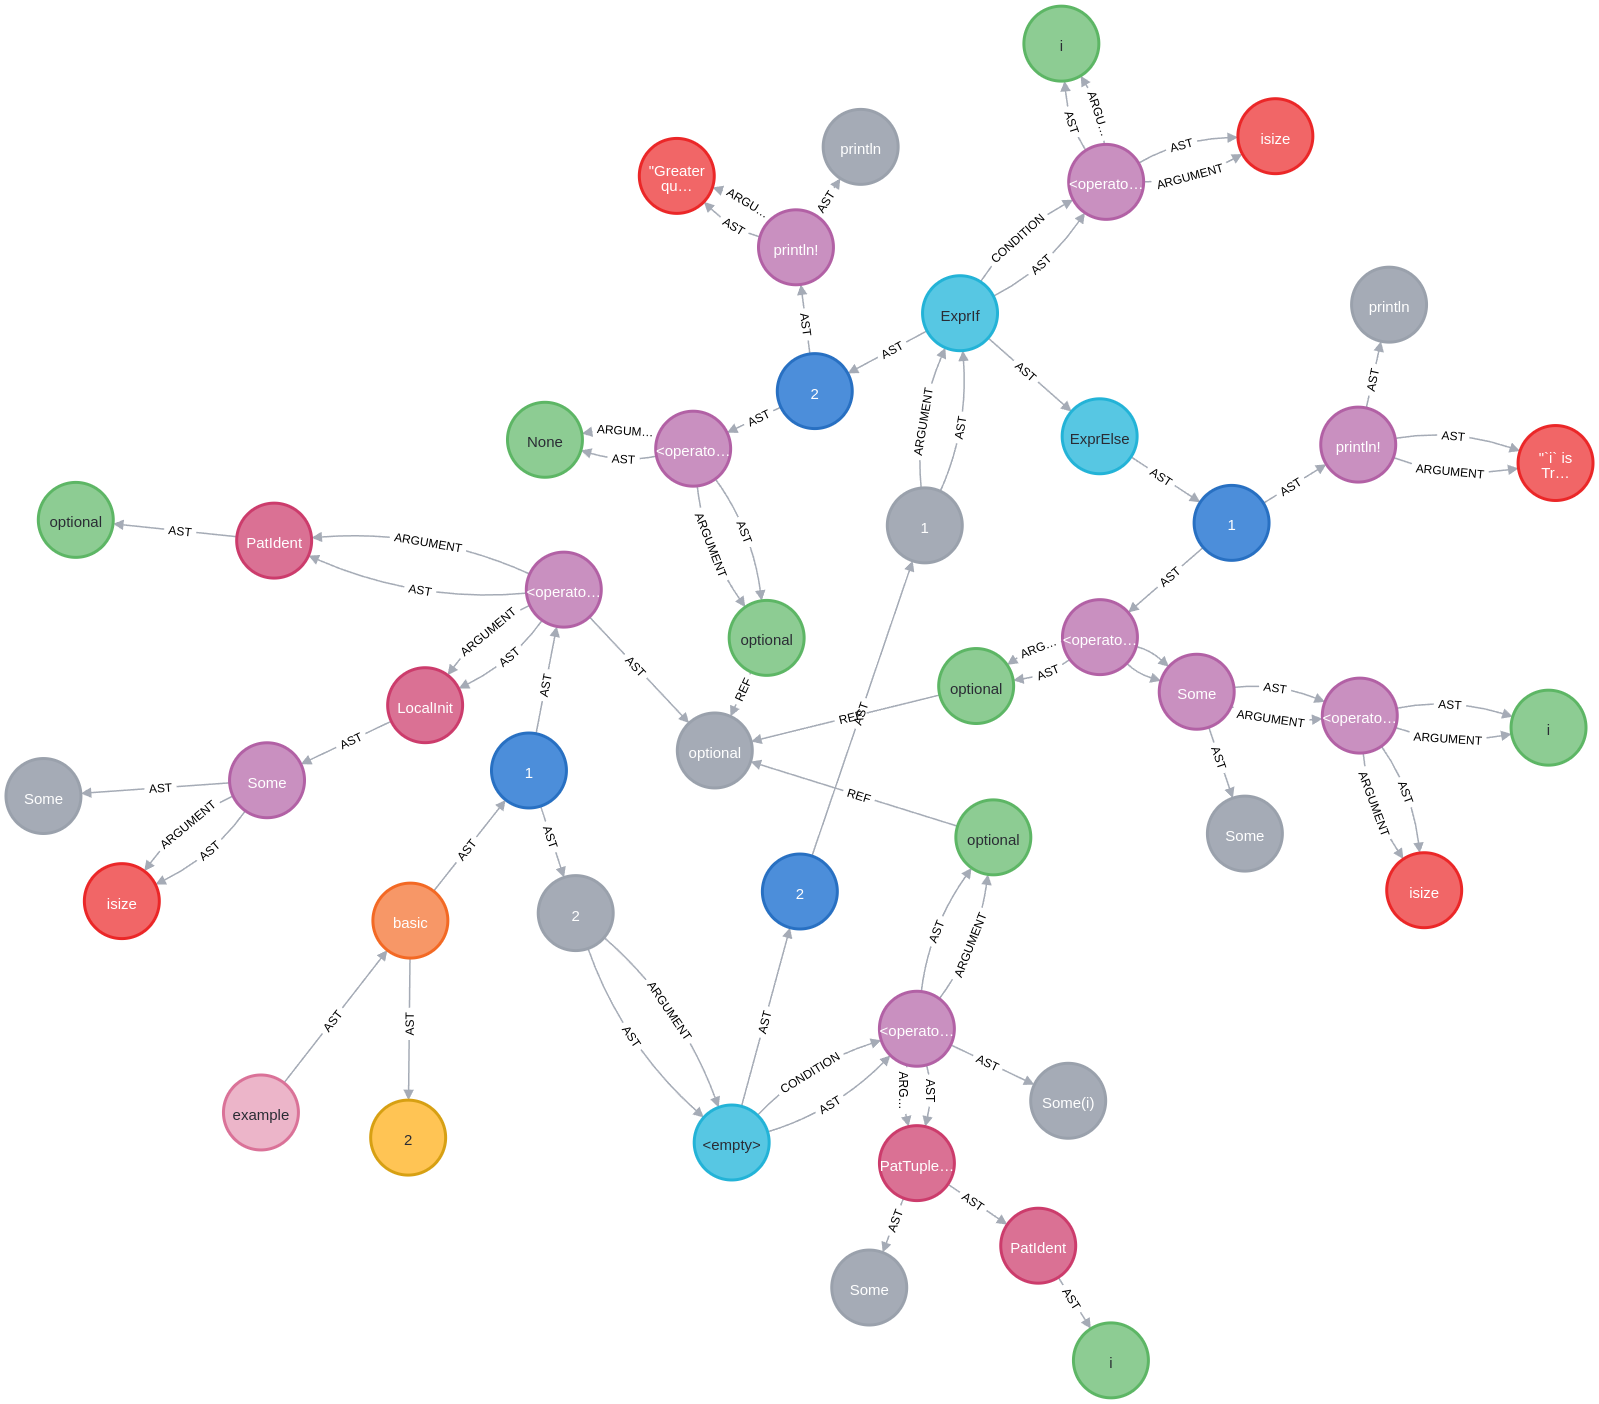
\includegraphics[width=1\columnwidth]{figures/c4/c4_whilelet.png}
    \centering
    \caption{Ví dụ đồ thị CPG cho đoạn mã nguồn while let \ref{code:c4_whilelet}}
    \label{img:c4_cpg_whilelet}
\end{figure}

\subsection{Cú pháp match}

Ngoài việc sử dụng mệnh đề gán biến thành biểu thức điều kiện, tính hướng hàm của Rust còn thể hiện ở tính năng match với sự kết hợp giữa Pattern matching và Algebraic Data Types.
Cấu trúc match không chỉ kiểm tra giá trị mà còn kết hợp với các pattern phức tạp, bao gồm kiểm tra điều kiện, kiểm tra các kiểu dữ liệu khác nhau và so sánh.
Điều này mang lại cho Rust tính linh hoạt cao hơn so với switch trong C/C++ khi chỉ so sánh giá trị nguyên thủy.

Một điểm khác biệt quan trọng giữa match và switch là tính toàn diện của match.
Rust yêu cầu các pattern trong match phải bao quát tất cả các khả năng có thể xảy ra, nếu không trình biên dịch sẽ báo lỗi.
Điều này giúp đảm bảo rằng không có tình huống nào bị bỏ qua, tăng cường độ an toàn của mã nguồn.
Trong khi đó, switch trong C/C++ không yêu cầu bao quát tất cả các trường hợp, và việc bỏ sót một trường hợp có thể dẫn đến lỗi hoặc hành vi không mong muốn.
Thêm vào đó, match trong Rust cho phép trích xuất và xử lý các thành phần của cấu trúc dữ liệu phức tạp ngay trong quá trình đối chiếu pattern.
Ví dụ, Rust có thể match trên \texttt{tuple}, \texttt{enum}, \texttt{struct}, trong khi switch của C/C++ thường chỉ giới hạn trong các giá trị nguyên thủy.

\begin{listing}[H]
\begin{minted}[mathescape, breaklines, frame=lines, framesep=2mm, baselinestretch=1.2, fontsize=\footnotesize, linenos]{rust}
enum Color {
    Red,
    Blue(u32, u32, u32),
    Green { red: u32, green: u32, blue: u32, },
}

fn main() {
    let color = Color::Blue(0, 0, 255);

    match color {
        Color::Red => println!("The color is Red!")
        Color::Blue(r, g, b) => println!("R: {}, G: {}, B: {}!", r, g, b)
        Color::Green {red, green, blue} => println!("R: {}, G: {}, B: {}!", red, green, blue),
    }
}
\end{minted}
\caption{Ví dụ mã nguồn cho match}
\label{code:c4_match}
\end{listing}

\begin{figure}[H]
    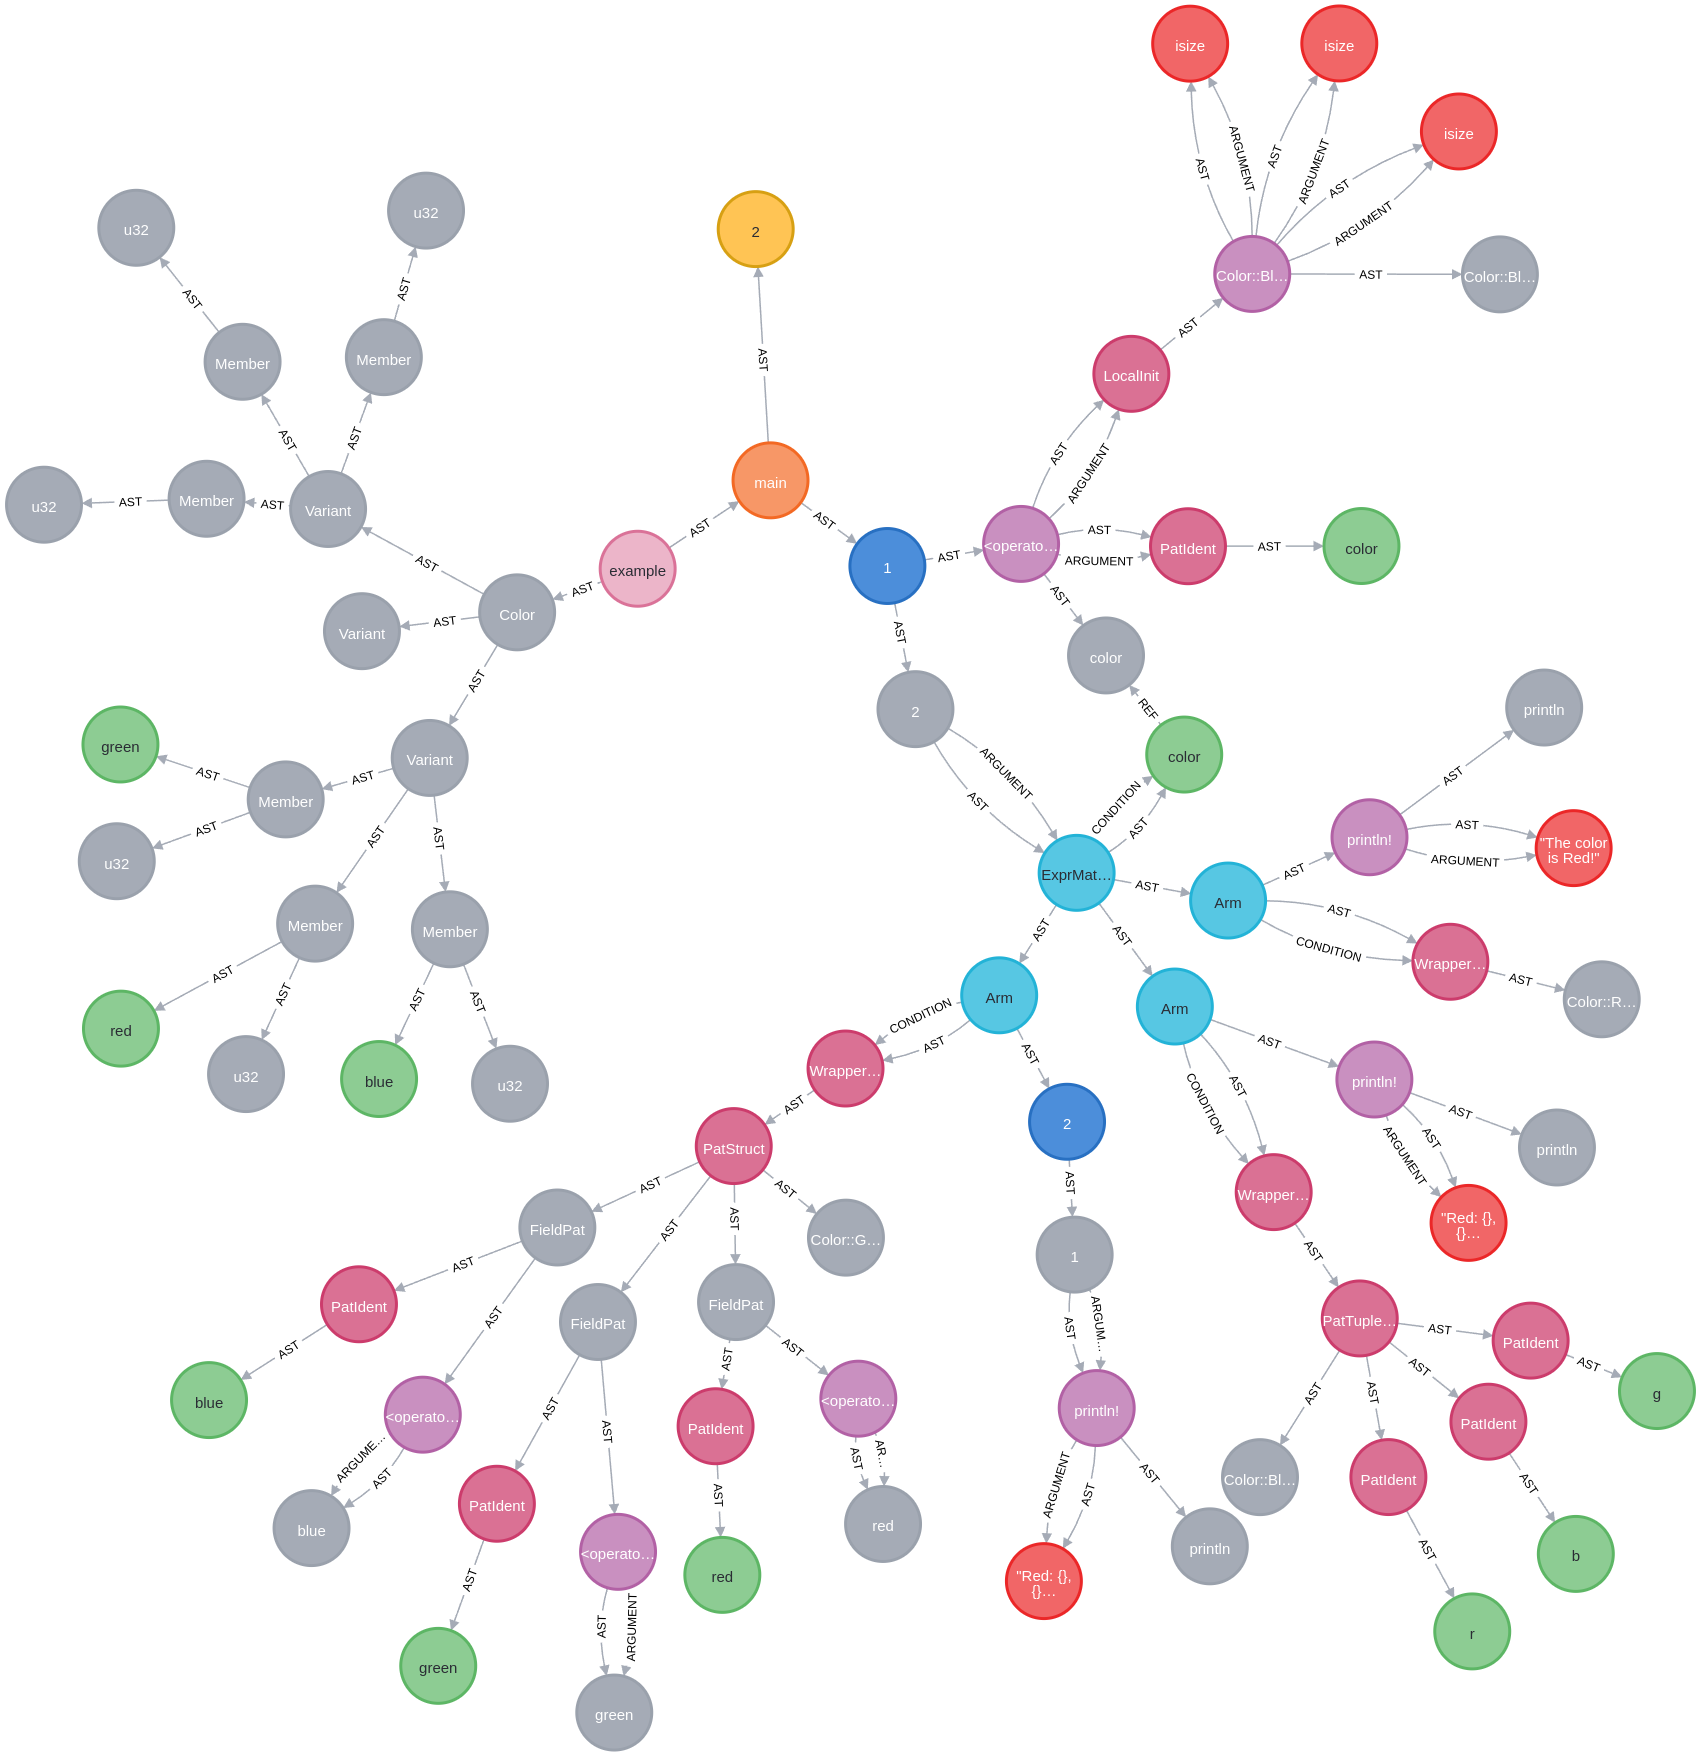
\includegraphics[width=1\columnwidth]{figures/c4/c4_match.png}
    \centering
    \caption{Ví dụ đồ thị CPG cho đoạn mã nguồn match \ref{code:c4_match}}
    \label{img:c4_match}
\end{figure}

\subsection{Cú pháp lifetime}

Lifetime là cơ chế được sử dụng trong Rust để quản lý vòng đời của các biến tham chiếu, đảm bảo rằng các biến tham chiếu không trỏ tới vùng nhớ không còn tồn tại.
Lifetime có vai trò tương tự như kiểu tổng quát, nhưng thay vì định kiểu cho biến thì lifetime sẽ xác định vòng đời cho biến tham chiếu.
Để biểu diễn được tính năng lifetime trên đồ thị CPG, có 3 loại nút mới được thêm vào đặc tả CPG là \texttt{Lifetime}, \texttt{LifetimeParameter}, \texttt{LifetimeArgument}.
Ngoài ra còn có cạnh \texttt{OUT\_LIVE} được bổ sung để chỉ ra quan hệ giữa biến và lifetime, quan hệ giữa các lifetime với nhau.

\texttt{LifetimeParameter} và \texttt{LifetimeArgument} được sử dụng cho các \texttt{struct}, \texttt{enum}, \texttt{trait} để chỉ ra lifetime tổng quát cho các biến tham chiếu.
Loại nút \texttt{Lifetime} sẽ thể hiện vòng đời thực sự của biến tham chiếu.
Các biến tham chiếu sẽ được gán lifetime thông qua việc sử dụng dấu "\texttt{'}" trước tên lifetime, ví dụ như \texttt{'a}.
Nếu các biến cùng đánh dấu lifetime \texttt{'a} thì sẽ có cạnh \texttt{OUT\_LIVE} trỏ từ biến tới nút \texttt{Lifetime} đại diện cho \texttt{'a} tương ứng.
Nếu lifetime \texttt{'a} được giới hạn bởi lifetime \texttt{'b} thì sẽ có cạnh \texttt{OUT\_LIVE} từ nút \texttt{Lifetime} \texttt{'a} tới nút \texttt{Lifetime} \texttt{'b}.

Ownership, borrowing và lifetime là 3 tính năng làm nên cơ chế an toàn bộ nhớ trong Rust.
Do vậy đồ thị CPG phải thể hiện được 3 tính năng trên đồ thị và cung cấp thông tin thông qua các nút, cạnh và thuộc tính phù hợp.
Đặc biệt là tính năng lifetime, vòng đời hợp lệ của các biến được thể hiện qua lifetime do đó việc thể hiện đúng quan hệ giữa lifetime và biến, lifetime với lifetime, biến với biến là rất quan trọng.
Từ đó có thể khai thác thông tin để kiểm tra vòng đời của biến tham chiếu, giúp phát hiện được các lỗi về bộ nhớ gây ra khi đánh dấu lifetime không chính xác.

% Lifetime elision là cơ chế trong Rust giúp tự động suy diễn lifetime cho các biến tham chiếu.
% Có ba luật chính về lifetime elision trong Rust.
% Thứ nhất, mỗi biến tham chiếu đầu vào sẽ được tự động gán lifetime mà không cần phải đánh dấu một cách tường minh.
% Thứ hai, nếu hàm có chỉ có một biến tham chiếu đầu và một biến tham chiếu đầu ra, trình biên dịch sẽ suy luận rằng biến tham chiếu đầu ra có cùng lifetime với biến tham chiếu đầu vào.
% Cuối cùng, nếu hàm có một hoặc nhiều hơn một biến tham chiếu đầu vào và một trong biến đầu vào là biến \texttt{self} (\texttt{self} tương đương với \texttt{this} trong C/C++), trình biên dịch sẽ suy luận rằng biến tham chiếu đầu ra có cùng lifetime với \texttt{self}.
% Ngoài 3 trường hợp trên, Rust yêu cầu phải ghi rõ lifetime cho tất cả các biến tham chiếu để tránh nhầm lẫn và đảm bảo an toàn bộ nhớ.

% \begin{listing}[H]
% \begin{minted}[mathescape, breaklines, frame=lines, framesep=2mm, baselinestretch=1.2, fontsize=\footnotesize, linenos]{rust}
% fn longest<'a>(x: &'a str, y: &'a str) -> &'a str {
%     if x.len() > y.len() {
%         x
%     } else {
%         y
%     }
% }
% \end{minted}
% \caption{Ví dụ mã nguồn cho lifetime cho hàm}
% \label{code:c4_lifetime_1}
% \end{listing}

% \begin{figure}[H]
%     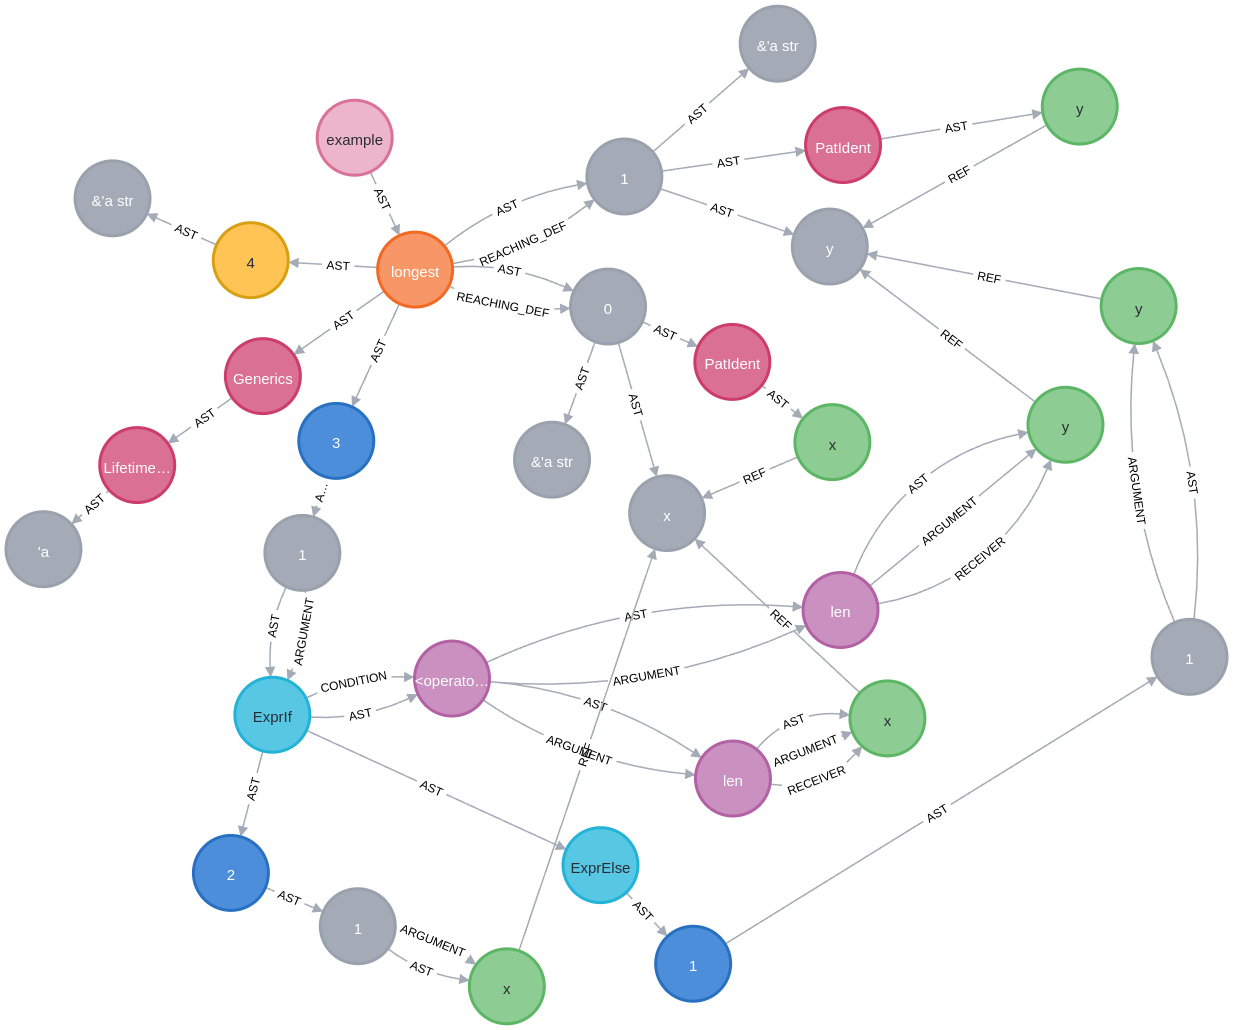
\includegraphics[width=1\columnwidth]{figures/c4/c4_lifetime_1.png}
%     \centering
%     \caption{Ví dụ đồ thị CPG cho đoạn mã nguồn \ref{code:c4_lifetime_1}}
%     \label{img:c4_lifetime_1}
% \end{figure}

\begin{listing}[H]
\begin{minted}[mathescape, breaklines, frame=lines, framesep=2mm, baselinestretch=1.2, fontsize=\footnotesize, linenos]{rust}
fn f<'a, 'b, 'c, 'd: 'c>(x: &'a i32, mut y: &'b i32, z: &'c i32)
where
    'a: 'b,
{
    // ...
}
\end{minted}
\caption{Ví dụ mã nguồn cho giới hạn lifetime}
\label{code:c4_lifetime_2}
\end{listing}

\begin{figure}[H]
    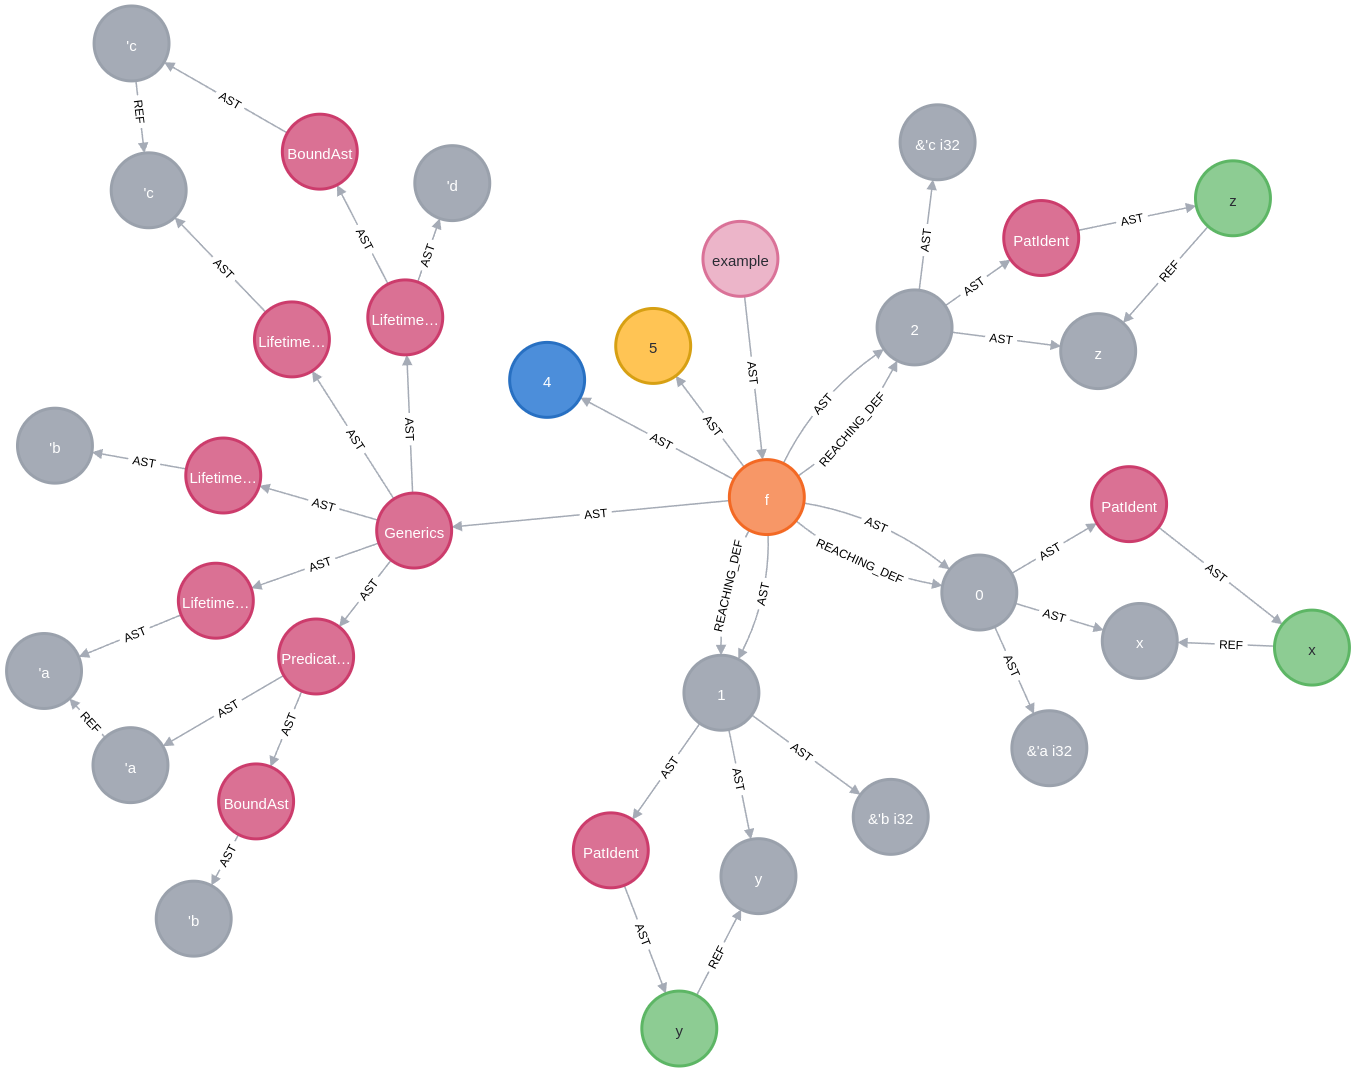
\includegraphics[width=1\columnwidth]{figures/c4/c4_lifetime_2.png}
    \centering
    \caption{Ví dụ đồ thị CPG cho đoạn mã nguồn \ref{code:c4_lifetime_2}}
    \label{img:c4_lifetime_2}
\end{figure}
